\documentclass{beamer}
\usepackage[english]{babel}
\usepackage[utf8]{inputenc}
\usepackage[T1]{fontenc}
\usepackage{graphicx}
\usepackage{listings}
\usepackage{color}

\definecolor{mygreen}{rgb}{0,0.6,0}
\definecolor{mygray}{rgb}{0.5,0.5,0.5}
\definecolor{mymauve}{rgb}{0.58,0,0.82}
\setlength\parindent{0pt}

\lstset{ %
  backgroundcolor=\color{white},   % choose the background color; you must add \usepackage{color} or \usepackage{xcolor}
  basicstyle=\tiny,        % the size of the fonts that are used for the code
  breakatwhitespace=false,         % sets if automatic breaks should only happen at whitespace
  breaklines=true,                 % sets automatic line breaking
  captionpos=b,                    % sets the caption-position to bottom
  commentstyle=\color{mygreen},    % comment style
  deletekeywords={...},            % if you want to delete keywords from the given language
  escapeinside={\%*}{*)},          % if you want to add LaTeX within your code
  extendedchars=true,              % lets you use non-ASCII characters; for 8-bits encodings only, does not work with UTF-8
  frame=none,	                   % adds a frame around the code
  keepspaces=true,                 % keeps spaces in text, useful for keeping indentation of code (possibly needs columns=flexible)
  keywordstyle=\color{blue},       % keyword style
  language=Octave,                 % the language of the code
  otherkeywords={*,...},           % if you want to add more keywords to the set
  numbers=left,                    % where to put the line-numbers; possible values are (none, left, right)
  numbersep=5pt,                   % how far the line-numbers are from the code
  numberstyle=\tiny\color{mygray}, % the style that is used for the line-numbers
  rulecolor=\color{black},         % if not set, the frame-color may be changed on line-breaks within not-black text (e.g. comments (green here))
  showspaces=false,                % show spaces everywhere adding particular underscores; it overrides 'showstringspaces'
  showstringspaces=false,          % underline spaces within strings only
  showtabs=false,                  % show tabs within strings adding particular underscores
  stepnumber=1,                    % the step between two line-numbers. If it's 1, each line will be numbered
  stringstyle=\color{mymauve},     % string literal style
  tabsize=2,	                   % sets default tabsize to 2 spaces
  title=\lstname                   % show the filename of files included with \lstinputlisting; also try caption instead of title
}

\usetheme{ENSLyon} 

\title[DM-Project 2]{French Presidential Election Candidates Tweets}
\author[E. Kerinec and N. Derumigny]{Emma Kerinec \and Nicolas Derumigny}
\institute[]{ENS Lyon}
\date{11 May 2017}


\usecolortheme{ENSLyon_blue}

\begin{document}

\begin{frame}
	\titlepage
	\begin{center}
	\end{center}
\end{frame}



\section{Introduction}
\begin{frame}{Introduction}
\begin{itemize}
\item Dataset: more than 3`000 tweets of the 11 French presidential election candidates.
\item Language: Python 3
\item Package: Sklearn, Numpy, Matplotlib
\end{itemize}

\end{frame}

\begin{frame}{Working on words}
\begin{block}{Preprocessing}
\begin{itemize}
\item Keep only relevant words $\to$ words whith more than 5 letters.
\item Distinguish hashtags with words.
\item Find common points between candidates without semantic analysis
\end{itemize}
\end{block}
\begin{itemize}
\item Hard to display on a graph $\to$ need a function $words \to \mathbb{R}$
\item Harder to see correlations
\end{itemize}
\end{frame}

\begin{frame}{Simple Data}
Compute the most used words for a given candidate.
\bigskip
\begin{figure}
\begin{columns}
\begin{column}{0.5\textwidth}
\begin{tabular}{ | c | c |}
\hline Word & Frequency\\
\hline
contre & 1.25\%\\
gouvernement & 0.49\%\\
travail & 0.45\%\\
paris & 0.40\%\\
droite & 0.38\%\\
solidarité &  0.38\%\\
\hline
\end{tabular}
\end{column}

\begin{column}{0.5\textwidth}
\begin{tabular}{ | c | c |}
\hline Hashtag & Frequency\\
\hline
\#npa & 11.03\%\\
\#loitravail & 2.98\%\\
\#grèce & 1.73\%\\
\#migrants & 1.66\%\\
\#poutou2017 & 1.45\%\\
\#hollande & 1.18\%\\
\hline
\end{tabular}
\end{column}
\end{columns}
\bigskip
\caption{Most used words and hashtags for Phillipe Poutou}
\end{figure}
\end{frame}


\section{Distance}
\begin{frame}{Distance between tweets}
\begin{block}{Distance of sets of words}
Measure the proportion of words that are different between two set of words $S_1$ and $S_2$:
\[
d(S_1, S_2)= \frac{1}{2} \cdot \Big( \sum_{\substack{w \in S_1\\w \notin S_2}}f(w) \quad + \quad \sum_{\substack{w \in S_2\\w \notin S_1}} f(w) \Big) 
\]
where $f(x)$ is the frequency of apparition of the word x.
\end{block}
\end{frame}

\begin{frame}{Distance between two candidates}
\begin{figure}

\begin{columns}
\begin{column}{.8\textwidth}
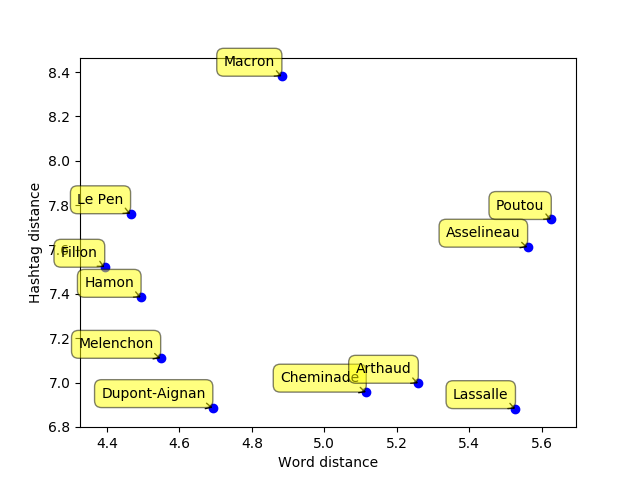
\includegraphics[width=\textwidth]{distances.png}
\end{column}

\begin{column}{.3\textwidth}
\caption{Sum of the distance to the other candidates, all words on $x$ and hashtags on $y$}
\end{column}
\end{columns}

\end{figure}
\end{frame}

\section{Data Mining}
\begin{frame}{Kmeans and Hierarchical clustering}
\begin{columns}
\begin{column}{.4\textwidth}
\center 
\begin{figure}
\begin{columns}
\begin{column}{.5\textwidth}
\center
Poutou\\
Cheminade\\
Arthaud\\
Lassalle\\
Asselineau\\
\end{column}


\begin{column}{.5\textwidth}
\center 
Melenchon\\
Fillon\\
Hamon\\
Le Pen\\
Macron\\
Dupont-Aignan
\end{column}
\end{columns}
\caption{Word Similarities}
\end{figure}
\end{column}


\vline

\begin{column}{.5\textwidth}
\center
\begin{figure}
\begin{columns}
\begin{column}{.5\textwidth}
\center
Macron
\end{column}

\begin{column}{.5\textwidth}
\center
Melenchon\\
Poutou\\
Fillon\\
Cheminade\\
Hamon\\
Arthaud\\
Le Pen\\
Lassalle\\
Asselineau\\
Dupont-Aignan
\end{column}
\end{columns}
\caption{Tweet Similarities}
\end{figure}
\end{column}
\end{columns}


\end{frame}

\begin{frame}{Variation over time}
Using Hierarchical clustering on hashtags.
\bigskip

\begin{columns}
\begin{column}{.4\textwidth}
\center 
\begin{figure}
\begin{columns}
\begin{column}{.5\textwidth}
\center
Fillon\\
Le Pen\\
Macron\\
Asselineau\\
Dupont-Aignan
\end{column}


\begin{column}{.5\textwidth}
\center 
Melenchon\\
Poutou\\
Cheminade\\
Hamon\\
Arthaud\\
Lassalle\\
\end{column}
\end{columns}
\caption{Before the campaign}
\end{figure}
\end{column}


\vline

\begin{column}{.5\textwidth}
\center
\begin{figure}
\begin{columns}
\begin{column}{.5\textwidth}
\center
Melenchon\\
Fillon\\
Hamon\\
Le Pen\\
Macron
\end{column}

\begin{column}{.5\textwidth}
\center
Poutou\\
Cheminade\\
Arthaud\\
Lassalle\\
Asselineau\\
Dupont-Aignan
\end{column}
\end{columns}
\caption{During the campaign}
\end{figure}
\end{column}
\end{columns}


\end{frame}

\begin{frame}{A priori algorithm}
\begingroup
\fontsize{9pt}{12pt}
\texttt{\\
Rule: ('\#fillon',) $\to$ ('français', 'dupontaignan') , 0.149\\
Rule: ('\#fillon', 'dlf\_officiel') $\to$ ('\#macron',) , 0.222\\
Rule: ('\#fillon', 'dlf\_officiel') $\to$ ('dupontaignan',) , 0.988\\
Rule: ('\#le79inter',) $\to$ ('dupontaignan',) , 1.000\\
Rule: ('\#legrandjury',) $\to$ ('dupontaignan',) , 1.000\\
...\\
Rule: ('judiciaire',) $\to$ ('casier',) , 0.937\\
Rule: ('judiciaire',) $\to$ ('vierge',) , 0.875\\
Rule: ('judiciaire',) $\to$ ('vierge', 'casier') , 0.875\\
Rule: ('élection',) $\to$ ('dupontaignan', 'dlf\_officiel') , 0.556\\
}
\endgroup


\begin{itemize}
\item Lots of auto-citations
\item Very few real expressions for the main candidates, except ``Front National''
\end{itemize}
\end{frame}


\section{Conclusion}
\begin{frame}{Conclusion}
\begin{center}
Thank you for listening. 
\bigskip


Does anybody have questions?
\end{center}
\end{frame}
 
\end{document}
